%%%%%%%%%%%%%%%%%%%%%%%%%%ch3-3
\begin{frame}[shrink]
  \frametitle{ch3.信号检测与估计理论的基础知识}
  \framesubtitle{ch3-3. 派生贝叶斯准则(1)}
  \tableofcontents[hideallsubsections]
\end{frame}

\begin{frame}{派生贝叶斯准则}
\begin{block}{基本要求}
	\begin{itemize} \setstretch{2.5}
		\item 掌握最小平均错误概率准则和最大后验概率准则
		\item 理解极小化极大准则和奈曼-皮尔逊准则的应用范围和基本原理
	\end{itemize}
\end{block}
\end{frame}

\section{最小平均错误概率准则}

\begin{frame}{最小平均错误概率准则}
\begin{block}{贝叶斯判决准则}
	\[ \frac{p(\bm{x}|H_1)}{p(\bm{x}|H_0)}\mathop{\gtrless}_{H_0}^{H_1}\frac{P(H_0)(c_{10}-c_{00})}{P(H_1)(c_{01}-c_{11})} \implies \lambda(\bm{x})\mathop{\gtrless}_{H_0}^{H_1}\eta \]
\end{block}
\begin{block}{最小平均错误概率准则}
	正确判决不付出代价, 错误判决代价相同。
	\[c_{01}=c_{10}=1, c_{00}=c_{11}=0\]
\end{block}
\end{frame}

\begin{frame}[shrink]{最小平均错误概率准则---判决域划分}
\begin{block}{最小平均错误概率准则}
	正确判决不付出代价, 错误判决代价相同。
	\[c_{01}=c_{10}=1, c_{00}=c_{11}=0\]
\end{block}
\begin{align*}
&C(H_0)=c_{00}P(H_0|H_0)+c_{10}P(H_1|H_0)=P(H_1|H_0)\\
&C(H_1)=c_{01}P(H_0|H_1)+c_{11}P(H_1|H_1)=P(H_0|H_1)\\
&\textbf{最小平均错误概率准则, 平均代价$C$}\Leftrightarrow\textbf{平均错误概率$P_e$}\\
C&=P(H_0)C(H_0)+P(H_1)C(H_1)\\
&=P(H_0)P(H_1|H_0)+P(H_1)P(H_0|H_1)
\end{align*}
\end{frame}

\begin{frame}[shrink]{最小平均错误概率准则---判决域划分}
\textbf{最小平均错误概率准则, 平均代价$C$}$\Leftrightarrow$\textbf{平均错误概率$P_e$}
\begin{columns}
	\column{0.5\textwidth}
	\small
	\begin{align*}
	C&=P(H_0)C(H_0)+P(H_1)C(H_1)\\
	&=P(H_0)P(H_1|H_0)+P(H_1)P(H_0|H_1)\\
	&=P(H_0)+\left(\int_{R_0}\left[P({H_1})p(\bm{x}|H_1)-P(H_0)p(\bm{x}|H_0)\right]dx \right)
	\end{align*}
    \scriptsize
	\textbf{把被积函数取负值的观测值$x$划分给$R_0$区域, 而把其余的观测值$x$划分给$R_1$, 即可保证平均代价最小。}
	\column{0.4\textwidth}
	\centering
	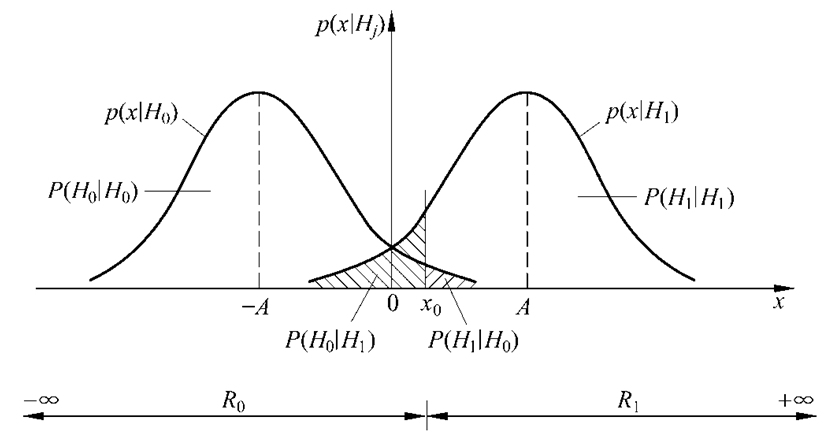
\includegraphics[scale=0.3]{detectionA}
	\scriptsize
	\begin{align*}
	P(H_1|H_0)&=1-\int_{R_0}p(x|H_0)dx\\ 
	P(H_0|H_1)&=\int_{R_0}p(x|H_1)dx
	\end{align*}
\end{columns}
\begin{align*}
&P({H_1})p(\bm{x}|H_1)< P(H_0)p(x|H_0)&\textbf{判决$H_0$假设成立}\\
&P({H_1})p(\bm{x}|H_1)\ge P(H_0)p(x|H_0)&\textbf{判决$H_1$假设成立}
\end{align*}
\end{frame}

\begin{frame}{最小平均错误概率准则}
\begin{block}{最小平均错误概率准则}
	\begin{align*}
	\frac{p(\bm{x}|H_1)}{p(\bm{x}|H_0)}&<\frac{P(H_0)}{P(H_1)}&\textbf{判决$H_0$假设成立}\\
	\frac{p(\bm{x}|H_1)}{p(\bm{x}|H_0)}&\ge\frac{P(H_0)}{P(H_1))}&\textbf{判决$H_1$假设成立}
	\end{align*}
	$\implies$
	\[ \lambda(\bm{x})\mathop{=}^{def}\frac{p(\bm{x}|H_1)}{p(\bm{x}|H_0)}\mathop{\gtrless}_{H_0}^{H_1}\frac{P(H_0)}{P(H_1)}\mathop{=}^{def}\eta \]
	$\implies$
	\[\ln\lambda(\bm{x})\mathop{\gtrless}_{H_0}^{H_1}\ln\eta \]
	$\implies$
	\[l(\bm{x})\mathop{\gtrless}_{H_0}^{H_1}\gamma \]
\end{block}
\end{frame}

\begin{frame}{最大似然检测准则}
\begin{block}{最小平均错误概率准则}
	\[ \lambda(\bm{x})\mathop{=}^{def}\frac{p(\bm{x}|H_1)}{p(\bm{x}|H_0)}\mathop{\gtrless}_{H_0}^{H_1}\frac{P(H_0)}{P(H_1)}\mathop{=}^{def}\eta \]
\end{block}
\begin{block}{最大似然检测准则}
	$c_{00}=c_{11}=0, c_{01}=c_{10}=1$, 且两个假设的先验概率等概, 则最小平均错误准则转化为最大似然检测准则。
	\[ p(\bm{x}|H_1)\mathop{\gtrless}_{H_0}^{H_1}p(\bm{x}|H_0) \]
\end{block}
\textbf{\textcolor{blue}{先验概率等概的最小平均错误概率准则为最大似然准则(maximum likelihood criterion)。}}
\end{frame}

\begin{frame}{贝叶斯准则例题5}
在闭启键控通信系统中,两个假设下的观测信号模型为:
\begin{align*}
H_0: x&=n  \\
H_1: x&=A+n
\end{align*}
其中, 噪声$n$是均值为零,方差为$\sigma_n^2$的高斯噪声,  若两个假设的先验概率相等, 且$c_{00}=c_{11}=0, c_{01}=c_{10}=1$。\\
~\\
采用最小平均错误概率准则, 试确定判决表示式, 并求最小平均错误概率。
\end{frame}

\begin{frame}[shrink]{贝叶斯准则例题5: 解}
解: 观测信号模型为:
\begin{align*}
H_0: x&=n  \\
H_1: x&=A+n
\end{align*}
由于, 先验概率等概的最小平均错误概率准则就是最大似然准则。 因此, 贝叶斯检测判别式为: 
	\[ p(x|H_1)\mathop{\gtrless}_{H_0}^{H_1}p(x|H_0)\implies \lambda(x)\mathop{=}^{def}\frac{p(x|H_1)}{p(x|H_0)}\mathop{\gtrless}_{H_0}^{H_1}1\mathop{=}^{def}\eta\]
由于$n$是高斯分布随机变量, 因此在$H_0$假设下, 检测统计量$x$服从高斯分布,且均值为0, 方差为$\sigma_n^2$; 在$H_1$假设下, 检测统计量$x$服从均值为$A$, 方差为$\sigma_n^2$的高斯分布。
\begin{align*}
&p(x|H_0)=\left(\frac{1}{2\pi\sigma_n^2}\right)^{1/2}\exp\left(-\frac{x^2}{2\sigma_n^2}\right) \qquad p(x|H_1)=\left(\frac{1}{2\pi\sigma_n^2}\right)^{1/2}\exp\left(-\frac{(x-A)^2}{2\sigma_n^2}\right)\\
&\lambda(x)=\frac{p(x|H_1)}{p(x|H_0)}=\exp\left(\frac{(x^2-(x-A)^2)}{2\sigma_n^2}\right)=\exp\left(\frac{A}{\sigma_n^2}x-\frac{A^2}{2\sigma_n^2}\right)
\end{align*} 
\end{frame}

\begin{frame}[shrink]{贝叶斯准则例题5: 解(续1)}
\begin{columns}
	\column{0.5\textwidth}
	\begin{align*}
	&\lambda(x)\mathop{=}^{def}\frac{p(x|H_1)}{p(x|H_0)}\mathop{\gtrless}_{H_0}^{H_1}1\mathop{=}^{def}\eta\\
	&\lambda(x)=\exp\left(\frac{A}{\sigma_n^2}x-\frac{A^2}{2\sigma_n^2}\right)\\
	&x\mathop{\gtrless}_{H_0}^{H_1}\frac{\sigma_n^2\ln\eta}{A}+\frac{A}{2}\mathop{=}^{def}\gamma
	\end{align*} 
	\column{0.5\textwidth}
	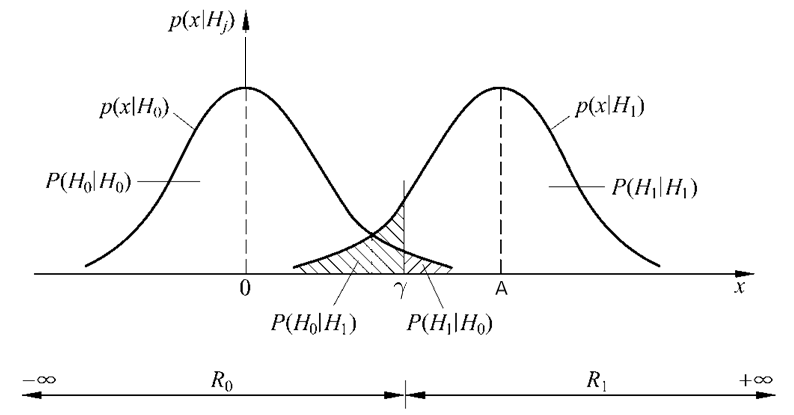
\includegraphics[scale=0.3]{0Ax}
\end{columns}
\begin{align*}
P(H_1|H_0)&=\int_{\gamma}^{\infty}p(x|H_0)dx\implies Q(x)=\int_{x}^{\infty}\left(\frac{1}{2\pi}\right)^{1/2}\exp\left(-\frac{u^2}{2}\right)du\\
&=\int_{\gamma}^{\infty}\left(\frac{1}{2\pi\sigma_n^2}\right)^{1/2}\exp\left(-\frac{x^2}{2\sigma_n^2}\right)dx\qquad 
&&\text{by } x=\sigma_nu\\
&=\int_{\frac{\gamma}{\sigma_n}}^{\infty}\left(\frac{1}{2\pi}\right)^{1/2}\exp\left(-\frac{u^2}{2}\right)du\qquad &&\text{by } \gamma=\frac{\sigma_n^2\ln\eta}{A}+\frac{A}{2}\\
&=\int_{\frac{\sigma_n\ln\eta}{A}+\frac{A}{2\sigma_n}}^{\infty}\left(\frac{1}{2\pi}\right)^{1/2}\exp\left(-\frac{u^2}{2}\right)du\qquad &&\text{by } d^2=\frac{A^2}{\sigma_n^2}\\
&=Q\left(\frac{\ln\eta}{d}+\frac{d}{2}\right)
\end{align*}
\end{frame}

\begin{frame}[shrink]{贝叶斯准则例题5: 解(续2)}
\begin{columns}
	\column{0.5\textwidth}
	\begin{align*}
	&\lambda(x)\mathop{=}^{def}\frac{p(x|H_1)}{p(x|H_0)}\mathop{\gtrless}_{H_0}^{H_1}1\mathop{=}^{def}\eta\\
	&\lambda(x)=\exp\left(\frac{A}{\sigma_n^2}x-\frac{A^2}{2\sigma_n^2}\right)\\
	&x\mathop{\gtrless}_{H_0}^{H_1}\frac{\sigma_n^2\ln\eta}{A}+\frac{A}{2}\mathop{=}^{def}\gamma
	\end{align*} 
	\column{0.5\textwidth}
	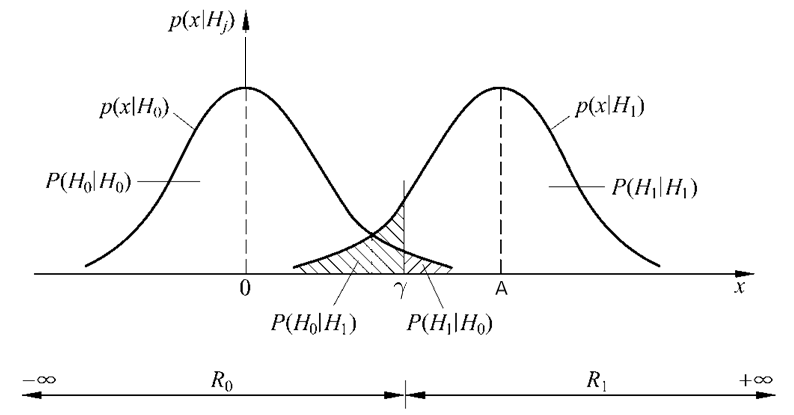
\includegraphics[scale=0.3]{0Ax}
\end{columns}
\begin{align*}
P(H_0|H_1)&=1-\int_{\gamma}^{\infty}p(x|H_1)dx\implies Q(x)=\int_{x}^{\infty}\left(\frac{1}{2\pi}\right)^{1/2}\exp\left(-\frac{u^2}{2}\right)du\\
&=1-\int_{\gamma}^{\infty}\left(\frac{1}{2\pi\sigma_n^2}\right)^{1/2}\exp\left(-\frac{(x-A)^2}{2\sigma_n^2}\right)dx\qquad 
&&\text{by } x=\sigma_nu+A\\
&=1-\int_{\frac{\gamma-A}{\sigma_n}}^{\infty}\left(\frac{1}{2\pi}\right)^{1/2}\exp\left(-\frac{u^2}{2}\right)du\qquad &&\text{by } \gamma=\frac{\sigma_n^2\ln\eta}{A}+\frac{A}{2}\\
&=1-\int_{\frac{\sigma_n\ln\eta}{A}-\frac{A}{2\sigma_n}}^{\infty}\left(\frac{1}{2\pi}\right)^{1/2}\exp\left(-\frac{u^2}{2}\right)du\qquad &&\text{by } d^2=\frac{A^2}{\sigma_n^2}\\
&=1-Q\left(\frac{\ln\eta}{d}-\frac{d}{2}\right)
\end{align*}
\end{frame}

\begin{frame}[shrink]{贝叶斯准则例题5: 解(续3)}
\begin{columns}
	\column{0.55\textwidth}
	\[\lambda(x)\mathop{=}^{def}\frac{p(x|H_1)}{p(x|H_0)}\mathop{\gtrless}_{H_0}^{H_1}1\mathop{=}^{def}\eta\implies\ln\eta=0\]
	\begin{align*}
	P(H_1|H_0)&=Q\left(\frac{\ln\eta}{d}+\frac{d}{2}\right)=Q\left(\frac{d}{2}\right)\\
	P(H_0|H_1)&=1-Q\left(\frac{\ln\eta}{d}-\frac{d}{2}\right)\\
	&=1-Q\left(-\frac{d}{2}\right)=Q\left(\frac{d}{2}\right)
	\end{align*}
	\column{0.45\textwidth}
	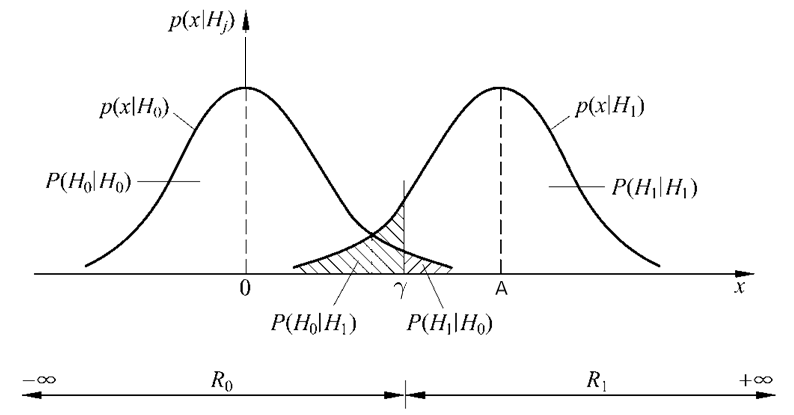
\includegraphics[scale=0.25]{0Ax}
\end{columns}
~\\
\textbf{最小平均错误概率准则, 平均代价$C$}$\Leftrightarrow$\textbf{平均错误概率$P_e$}, $P(H_0)=P(H_1)=\frac{1}{2}$
\begin{align*}
P_e=C&=P(H_0)P(H_1|H_0)+P(H_1)P(H_0|H_1)\\
&=\frac{1}{2}Q\left(\frac{d}{2}\right)+\frac{1}{2}Q\left(\frac{d}{2}\right)=Q\left(\frac{d}{2}\right)\qquad d^2=\frac{A^2}{\sigma_n^2}
\end{align*}
\textbf{\textcolor{blue}{$Q(x)$是单调递减函数, 信噪比d越高, 平均错误概率越小, 检测性能越好。
}}
\end{frame}

\begin{frame}[shrink]{标准高斯分布的右尾积分}
\begin{columns}
	\column{0.5\textwidth}
	\begin{align*}
	&Q(x)=\int_{x}^{\infty}\left(\frac{1}{2\pi}\right)^{1/2}\exp\left(-\frac{u^2}{2}\right)du\\
	&Q\left(\frac{d}{2}\right) = 1-Q\left(-\frac{d}{2}\right)
	\end{align*}
	\column{0.5\textwidth}
	\centering
	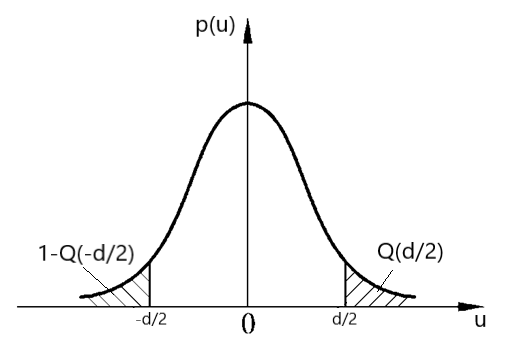
\includegraphics[scale=0.4]{Qdd}
\end{columns}
\end{frame}

\section{最大后验概率准则}

\begin{frame}[shrink]{最大后验概率准则}
\begin{block}{贝叶斯判决准则}
	\[ \frac{p(\bm{x}|H_1)}{p(\bm{x}|H_0)}\mathop{\gtrless}_{H_0}^{H_1}\frac{P(H_0)(c_{10}-c_{00})}{P(H_1)(c_{01}-c_{11})} \implies \lambda(\bm{x})\mathop{\gtrless}_{H_0}^{H_1}\eta \]
\end{block}
\begin{block}{最大后验概率准则}
	代价因子满足: $c_{10}-c_{00}=c_{01}-c_{11}$\\
	判决表示式
	\[ \frac{p(\bm{x}|H_1)}{p(\bm{x}|H_0)}\mathop{\gtrless}_{H_0}^{H_1}\frac{P(H_0)}{P(H_1)} \]
\end{block}
\begin{block}{Notes}
	\small
	\begin{itemize}
		\item 最大后验概率准则形式上与最小平均错误概率准则相同
		\item 问题: 可写成上述判决表达式形式的, 是否一定可以获得
		最小平均错误概率?
	\end{itemize}
\end{block}
\end{frame}

\begin{frame}[shrink]{最大后验概率准则不一定能获得最小平均错误概率}
\begin{block}{最大后验概率准则}
	代价因子满足: $c_{10}-c_{00}=c_{01}-c_{11}$\\
	判决表示式
	\[ \frac{p(\bm{x}|H_1)}{p(\bm{x}|H_0)}\mathop{\gtrless}_{H_0}^{H_1}\frac{P(H_0)}{P(H_1)} \]
\end{block}
\begin{block}{Notes}
	最小平均错误概率准则: $c_{01}=c_{10}=1, c_{00}=c_{11}=0$。\\ 
	可得到最小平均错误概率:
	\begin{align*}
	P_e=C=P(H_0)C(H_0)+P(H_1)C(H_1)=P(H_0)P(H_1|H_0)+P(H_1)P(H_0|H_1)
	\end{align*}
	因此, 虽然最大后验概率准则形式上与最小平均错误概率准则相同。但是不一定能获得最小平均错误概率?
\end{block}
\end{frame}

\begin{frame}[shrink]{最大后验概率准则}
在贝叶斯准则中, 当代价因子满足: $c_{10}-c_{00}=c_{01}-c_{11}$时 
\[\lambda(\bm{x})=\frac{p(\bm{x}|H_1)}{p(\bm{x}|H_0)}\mathop{\gtrless}\limits_{H_0}^{H_1}\frac{P(H_0)}{P(H_1)}\implies P(H_1)p(\bm{x}|H_1)\mathop{\gtrless}\limits_{H_0}^{H_1}P(H_0)p(\bm{x}|H_0)\]
由条件概率公式$P(A|B)=\frac{P(AB)}{P(B)}$,有
\[P(H_1|(\bm{x}\le X\le \bm{x}+d\bm{x}))=\frac{P((\bm{x}\le X\le \bm{x}+d\bm{x})|H_1)P(H_1)}{P(\bm{x}\le X\le \bm{x}+d\bm{x})}\]
当$d\bm{x}$很小时,有$P(H_1|(\bm{x}\le X\le \bm{x}+d\bm{x}))=P(H_1|\bm{x})$, $P((\bm{x}\le X\le \bm{x}+d\bm{x})|H_1)=p(\bm{x}|H_1)d\bm{x},\quad P(\bm{x}\le X\le \bm{x}+d\bm{x})=p(\bm{x})d\bm{x}$\\
从而得
\[P(H_1|\bm{x})=\frac{p(\bm{x}|H_1)d\bm{x}P(H_1)}{p(\bm{x})d\bm{x}}=\frac{p(\bm{x}|H_1)P(H_1)}{p(\bm{x})}\]
\[\implies P(H_1)p(\bm{x}|H_1)=p(\bm{x})P(H_1|\bm{x}) \]
类似地,可得
\[P(H_0)p(\bm{x}|H_0)=p(\bm{x})P(H_0|\bm{x}) \]
\end{frame}

\begin{frame}[shrink]{最大后验概率准则}
\[P(H_1)p(\bm{x}|H_1)=p(\bm{x})P(H_1|\bm{x}),\quad P(H_0)p(\bm{x}|H_0)=p(\bm{x})P(H_0|\bm{x}) \]
\[\lambda(\bm{x})=\frac{p(\bm{x}|H_1)}{p(\bm{x}|H_0)}\mathop{\gtrless}\limits_{H_0}^{H_1}\frac{P(H_0)}{P(H_1)}\implies P(H_1)p(\bm{x}|H_1)\mathop{\gtrless}\limits_{H_0}^{H_1}P(H_0)p(\bm{x}|H_0)\]
\[p(\bm{x})P(H_1|\bm{x})\mathop{\gtrless}\limits_{H_0}^{H_1}p(\bm{x})P(H_0|\bm{x}) \]
\[P(H_1|\bm{x})\mathop{\gtrless}\limits_{H_0}^{H_1}P(H_0|\bm{x}) \]
$P(H_j|\bm{x})(j=0,1)$表示已经获得观测量$\bm{x}$的条件下,假设$H_j$为真时的概率, 称为\textbf{后验概率}。\\
按照最小平均代价的贝叶斯准则在代价因子满足: $c_{10}-c_{00}=c_{01}-c_{11}$时,就成为\textbf{最大后验概率准则(maximum a posteriori probability criterion)} 
\end{frame}

\begin{frame}[shrink]{贝叶斯准则以及派生贝叶斯准则}
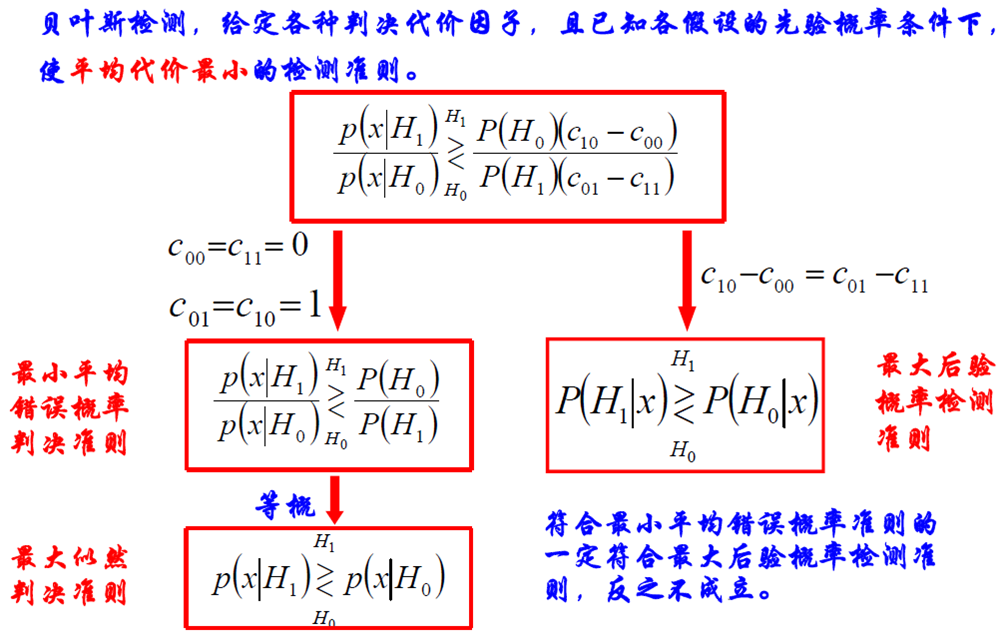
\includegraphics[scale=0.5]{bys}
\end{frame}

\section{极小极大化准则和奈曼皮尔逊准则}

\begin{frame}[shrink]{极小极大化准则和奈曼皮尔逊准则}
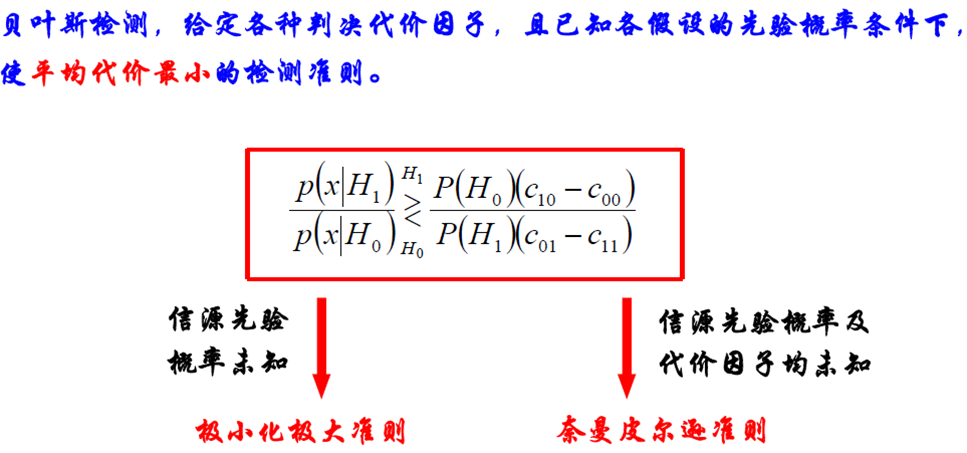
\includegraphics[scale=0.5]{minimax-NP}
\end{frame}

\begin{frame}[shrink]{极小极大化准则}
\begin{block}{贝叶斯判决准则}
	\[ \frac{p(\bm{x}|H_1)}{p(\bm{x}|H_0)}\mathop{\gtrless}_{H_0}^{H_1}\frac{P(H_0)(c_{10}-c_{00})}{P(H_1)(c_{01}-c_{11})} \implies \lambda(\bm{x})\mathop{\gtrless}_{H_0}^{H_1}\eta \]
\end{block}
\begin{block}{极小极大化准则}
	\begin{itemize}
		\setlength{\itemsep}{.5cm}
		\item 应用范围:\\
		假设的先验概率未知,判决代价因子给定
		\item 目的:\\
		尽可能避免产生过分大的代价,使极大可能代价最小化
	\end{itemize}
\end{block}
\end{frame}

\begin{frame}[shrink]{极小极大化准则}
\begin{itemize} 
	\setlength{\itemsep}{.5cm}
	\item 在先验概率未知的情况下, 平均代价的性质?\\
	\textbf{\textcolor{blue}{平均代价是先验概率的函数}}
	\[C=P(H_0)C(H_0)+P(H_1)C(H_1)\]
	\item 在先验概率未知的情况下, 进行检测的方法是:\\
	\textbf{\textcolor{blue}{先假设一个先验概率$P_{1g}$, 然后按照贝叶斯准则进行检测。}}
	\item 为尽可能降低代价, 需设计一种先验概率的假设方法, 使由此得到的检测准则的带价值与先验概率无关。\\
	\textbf{\textcolor{blue}{尽可能避免产生过分大的代价, 使极大可能代价最小化。}}
\end{itemize}
\end{frame}

\begin{frame}{几种符号定义}
\begin{columns}
	\column{0.5\textwidth}
	\begin{align*}
	&H_0: x=n &&\text{仅含噪声信号}\\
	&H_1: x=A+n &&\text{雷达检测回波信号}
	\end{align*}
	\column{0.5\textwidth}
	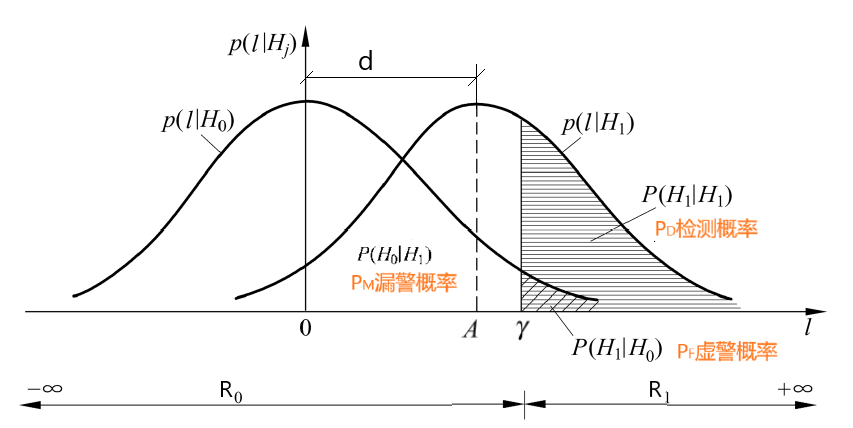
\includegraphics[scale=0.25]{R0R1}
\end{columns}
\begin{itemize}
	\setlength{\itemsep}{.2cm}
	\item \textbf{\textcolor{blue}{虚警概率}}$P_F\mathop{=}\limits^{def}P(H_1|H_0)$: False alarm, 假设$H_0$为真的条件下,判决$H_1$成立的概率。是个假判决。
	\item \textbf{\textcolor{blue}{漏警概率}}$P_M\mathop{=}\limits^{def}P(H_0|H_1)$: Miss alarm, 假设$H_1$为真的条件下, 判决$H_0$成立的概率。是个遗漏的判决。
	\item \textbf{\textcolor{blue}{检测概率}}$P_D\mathop{=}\limits^{def}P(H_1|H_1)$: Ditection alarm, 假设$H_1$为真的条件下, 判决$H_1$成立的概率。是个正确检测的判决。
\end{itemize}
\end{frame}

\begin{frame}{几种符号定义(续)}
\begin{columns}
	\column{0.5\textwidth}
	\begin{align*}
	&H_0: x=n &&\text{仅含噪声信号}\\
	&H_1: x=A+n &&\text{雷达检测回波信号}
	\end{align*}
	\column{0.5\textwidth}
	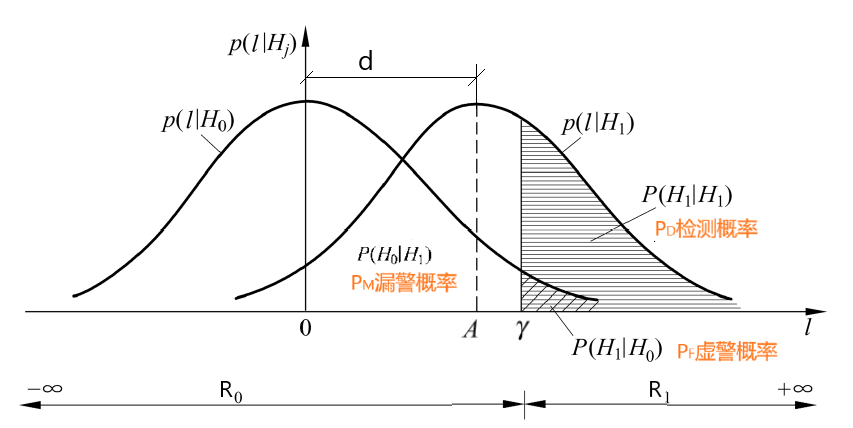
\includegraphics[scale=0.25]{R0R1}
\end{columns}
\begin{align*}
&\textbf{\textcolor{blue}{虚警概率}}
&&P_F\mathop{=}\limits^{def}P(H_1|H_0)=\int_{R_1}p(\bm{x}|H_0)d\bm{x}=1-\int_{R_0}p(\bm{x}|H_0)d\bm{x}\\
&\textbf{\textcolor{blue}{漏警概率}}
&&P_M\mathop{=}\limits^{def}P(H_0|H_1)=\int_{R_0}p(\bm{x}|H_1)d\bm{x}\\
&\textbf{\textcolor{blue}{检测概率}}
&&P_D\mathop{=}\limits^{def}P(H_1|H_1)=\int_{R_1}p(\bm{x}|H_1)d\bm{x}\\
&\textbf{\textcolor{blue}{先验概率}}
&&P_1\mathop{=}^{def}P(H_1)=1-P(H_0)\mathop{=}^{def}=1-P_0
\end{align*}
\end{frame}

\begin{frame}[shrink]{极小极大化准则---先验概率未知, 平均代价的性质}
\begin{itemize} 
	%\setlength{\itemsep}{.5cm}
	\item 先验概率和代价因子已知时, 平均代价为
	\begin{align*}
	C&=P(H_0)C(H_0)+P(H_1)C(H_1)\\
	&=P(H_0)(c_{00}P(H_0|H_0)+c_{10}P(H_1|H_0))+P(H_1)(c_{01}P(H_0|H_1)+c_{11}P(H_1|H_1))
	\end{align*}
	\item 代价因子已知, 先验概率未知时,\textbf{\textcolor{blue}{平均代价是先验概率的函数。}} $P_1\mathop{=}\limits^{def}P(H_1)$
    \begin{align*}
    C(P_1)&=(1-P(H_1))(c_{00}P(H_0|H_0)+c_{10}P(H_1|H_0))+P(H_1)(c_{01}P(H_0|H_1)+c_{11}P(H_1|H_1))\\
    &=(1-P_1)(c_{00}P(H_0|H_0)+c_{10}P(H_1|H_0))+P_1(c_{01}P(H_0|H_1)+c_{11}P(H_1|H_1))
    \end{align*}
	\item 先验概率未知时,由于贝叶斯判决门限是先验概率$P_1$的函数, 因此\textbf{\textcolor{blue}{漏警概率$P_M$和虚警概率$P_F$也是先验概率$P_1$的函数。}}
\end{itemize}
\begin{align*}
&\eta\mathop{=}^{def}\eta(P_1)=\frac{P(H_0)(c_{10}-c_{00})}{P(H_1)(c_{01}-c_{11})}=\frac{(1-P_1)(c_{10}-c_{00})}{P_1(c_{01}-c_{11})}=\frac{1}{P_1(c_{01}-c_{11})}-\frac{c_{10}-c_{00}}{c_{01}-c_{11}}\\
&P_M(P_1)\mathop{=}^{def}P(H_0|H_1)=\int_{R_0}p(x|H_1)dx,\quad P_F(P_1)\mathop{=}^{def}P(H_1|H_0)=\int_{R_1}p(x|H_0)dx
\end{align*}
\end{frame}

\begin{frame}[shrink]{极小极大化准则---先验概率未知, 平均代价的性质}
\small
\begin{columns}
	\column{0.5\textwidth}
	\begin{align*}
	&P_1\mathop{=}\limits^{def}P(H_1),\quad P_M(P_1)\mathop{=}^{def}P(H_0|H_1),\quad P_F(P_1)\mathop{=}^{def}P(H_1|H_0)\\
	&P(H_1|H_1)=1-P(H_0|H_1)=1-P_M(P_1)\\
	&P(H_0|H_0)=1-P(H_1|H_0)=1-P_F(P_1)
	\end{align*}
	\column{0.4\textwidth}
	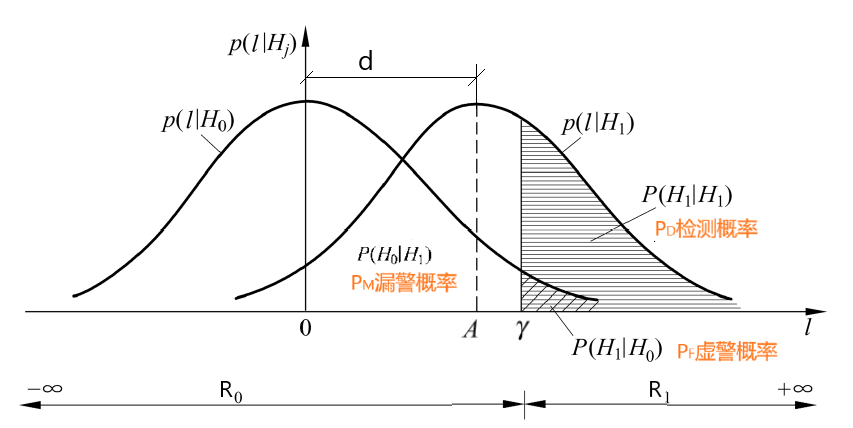
\includegraphics[scale=0.22]{R0R1}
\end{columns}
\begin{align*}
	C(P_1)&=(1-P(H_1))(c_{00}P(H_0|H_0)+c_{10}P(H_1|H_0))+P(H_1)(c_{01}P(H_0|H_1)+c_{11}P(H_1|H_1))\\
	&=(1-P_1)(c_{00}P(H_0|H_0)+c_{10}P(H_1|H_0))+P_1(c_{01}P(H_0|H_1)+c_{11}P(H_1|H_1))\\
	&=(1-P_1)(c_{00}(1-P_F(P_1))+c_{10}P_F(P_1))+P_1(c_{01}P_M(P_1)+c_{11}(1-P_M(P_1))\\
	&=(1-P_1)c_{00}+(1-P_1)(c_{10}-c_{00})P_F(P_1)+P_1c_{11}+P_1(c_{01}-c_{11})P_M(P_1)\\
	&=c_{00}-P_1c_{00}+(c_{10}-c_{00})P_F(P_1)-P_1(c_{10}-c_{00})P_F(P_1)+P_1c_{11}+P_1(c_{01}-c_{11})P_M(P_1)\\
	&=c_{00}+(c_{10}-c_{00})P_F(P_1)\\
	&+P_1[(c_{11}-c_{00})+(c_{01}-c_{11})P_M(P_1)-(c_{10}-c_{00})P_F(P_1)]
\end{align*}
\end{frame}

\begin{frame}[shrink]{极小极大化准则---先验概率未知, 平均代价的性质}
\begin{columns}
	\small
	\column{0.5\textwidth}
	\begin{align*}
	&P_1\mathop{=}\limits^{def}P(H_1),\quad P_M(P_1)\mathop{=}^{def}P(H_0|H_1),\quad P_F(P_1)\mathop{=}^{def}P(H_1|H_0)\\
	&P(H_1|H_1)=1-P(H_0|H_1)=1-P_M(P_1)\\
	&P(H_0|H_0)=1-P(H_1|H_0)=1-P_F(P_1)\\
	&\eta\mathop{=}^{def}\eta(P_1)=\frac{1}{P_1(c_{01}-c_{11})}-\frac{c_{10}-c_{00}}{c_{01}-c_{11}}
	\end{align*}
	\column{0.4\textwidth}
	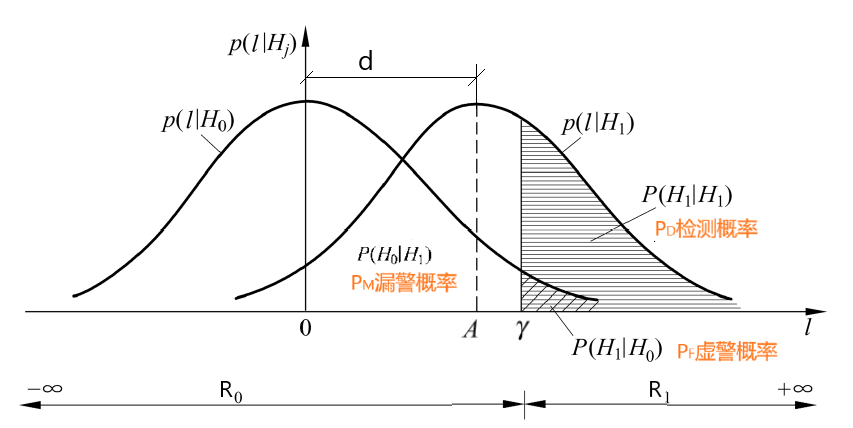
\includegraphics[scale=0.22]{R0R1}
\end{columns}
~\\
\textbf{\textcolor{blue}{当$\lambda(\bm{x})$是严格单调的概率分布随机变量时,平均代价$C(P_1)$是先验概念率$P_1$的严格上凸函数。}}
\begin{columns}
	\column{0.7\textwidth}
	\begin{align*}
	C(P_1)&=c_{00}+(c_{10}-c_{00})P_F(P_1)\\
	&+P_1[(c_{11}-c_{00})+(c_{01}-c_{11})P_M(P_1)-(c_{10}-c_{00})P_F(P_1)]\\
	&P_1\uparrow\implies \eta\downarrow, P_M\downarrow, P_F\uparrow, P_D\uparrow, C\uparrow\sim C_{minmax}\sim\downarrow
	\end{align*}
	~\\
	\column{0.3\textwidth}
	\centering
	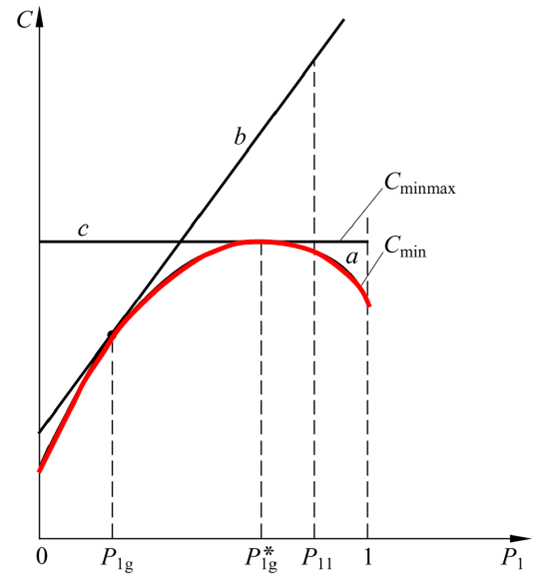
\includegraphics[scale=0.22]{C-P1}
\end{columns}
\end{frame}

\begin{frame}[shrink]{极小极大化准则}
\textbf{目的: 尽可能避免产生过分大的代价,使极大可能代价最小化。}
\begin{enumerate}
	\item 猜测一个先验概率$P_{1g}$, 以$\eta(P_{1g})$为门限进行判决。
	\item $P_{1g}$确定, $P_M(P_{1g})$和$P_F(P_{1g})$即可确定。
	\item $P_{1g}$确定,则$C(P_1,P_{1g})$表示与上凸函数曲线$C(P_1)$的切线,如图中的直线$b$, $c$。
\end{enumerate}
\begin{columns}
	\column{0.7\textwidth}
	\begin{align*}
	&\eta\mathop{=}^{def}\eta(P_{1g})=\frac{1}{P_{1g}(c_{01}-c_{11})}-\frac{c_{10}-c_{00}}{c_{01}-c_{11}}\\
	&C(P_1)=c_{00}+(c_{10}-c_{00})P_F(P_1)+\\
	&P_1[(c_{11}-c_{00})+(c_{01}-c_{11})P_M(P_1)-(c_{10}-c_{00})P_F(P_1)]\\
	&C(P_1,P_{1g})=c_{00}+(c_{10}-c_{00})P_F(P_{1g})+\\
	&P_1[(c_{11}-c_{00})+(c_{01}-c_{11})P_M(P_{1g})-(c_{10}-c_{00})P_F(P_{1g})]
	\end{align*}
	\column{0.3\textwidth}
	\centering
	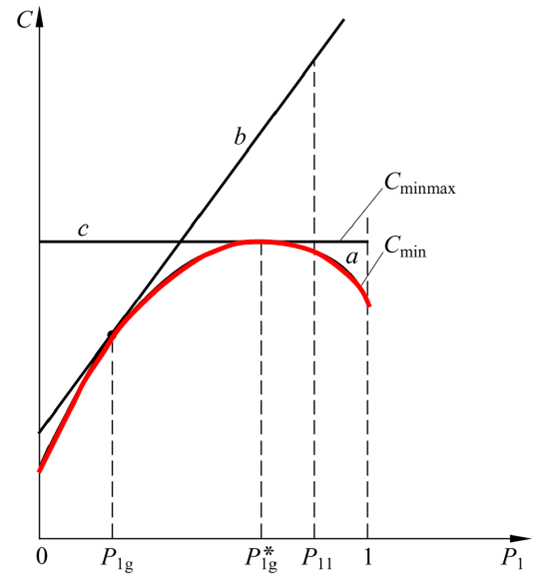
\includegraphics[scale=0.25]{C-P1}
\end{columns}
\end{frame}

\begin{frame}[shrink]{极小极大化准则}
\textbf{目的: 尽可能避免产生过分大的代价,使极大可能代价最小化。}
\begin{enumerate}
\setcounter{enumi}{3}
\item 如果实际$P_1=P_{1g}$, 平均代价最小, 在直线$b$与$C(P_1)$的切点处, $C(P_1=P_{1g},P(_{1g}))$。
\item 如果实际$P_1\ne P_{1g}$, 比如$P_1=P_{11}$, 则平均代价远大于$C(P_1=P_{1g},P(_{1g}))$, 在直线$P_1=P_{11}$与直线$b$的交点处。
\item 如果猜测的先验概率为$P_{1g}^{\ast}$,则无论实际的先验概率$P_1$为多大,平均代价都等于$C_{minmax}$, 而不会产生过分大的代价。\textbf{\textcolor{blue}{产生的代价与先验概率$P_1$无关。$P_{1g}^{\ast}$即是先验概率$P_1$最理想的猜测值。}}
\end{enumerate}
\begin{columns}
\column{0.7\textwidth}
\begin{align*}
&C(P_1,P_{1g})=c_{00}+(c_{10}-c_{00})P_F(P_{1g})+\\
&P_1[(c_{11}-c_{00})+(c_{01}-c_{11})P_M(P_{1g})-(c_{10}-c_{00})P_F(P_{1g})]
\end{align*}
~\\
\column{0.3\textwidth}
\centering
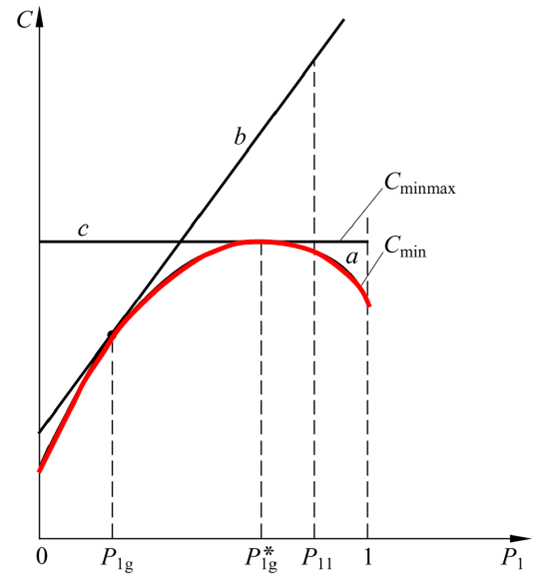
\includegraphics[scale=0.18]{C-P1}
\end{columns}
\end{frame}

\begin{frame}[shrink]{极小极大化准则}
先验概率未知的情况下, 可猜测一个先验概率$P_{1g}$, 然后利用贝叶斯准则进行检测。
判决门限是$P_{1g}$的函数,判决区域$R_0$是$P_{1g}$的函数, 判决区域$R_1$是$P_{1g}$的函数
\begin{columns}
	\column{0.7\textwidth}
	\begin{align*}
	&\eta\mathop{=}^{def}\eta(P_{1g})=\frac{1}{P_{1g}(c_{01}-c_{11})}-\frac{c_{10}-c_{00}}{c_{01}-c_{11}}\\
	&P_M=\int_{R_0}p(x|H_1)dx\mathop{=}^{def}P_M(P_{1g}), P_F=\int_{R_1}p(x|H_0)dx\mathop{=}^{def}P_F(P_{1g})\\
	&C(P_1)=c_{00}+(c_{10}-c_{00})P_F(P_1)+\\
	&P_1[(c_{11}-c_{00})+(c_{01}-c_{11})P_M(P_1)-(c_{10}-c_{00})P_F(P_1)]\\
	&C(P_1,P_{1g})=c_{00}+(c_{10}-c_{00})P_F(P_{1g})+\\
	&P_1[(c_{11}-c_{00})+(c_{01}-c_{11})P_M(P_{1g})-(c_{10}-c_{00})P_F(P_{1g})]
	\end{align*}
	\column{0.3\textwidth}
	\centering
	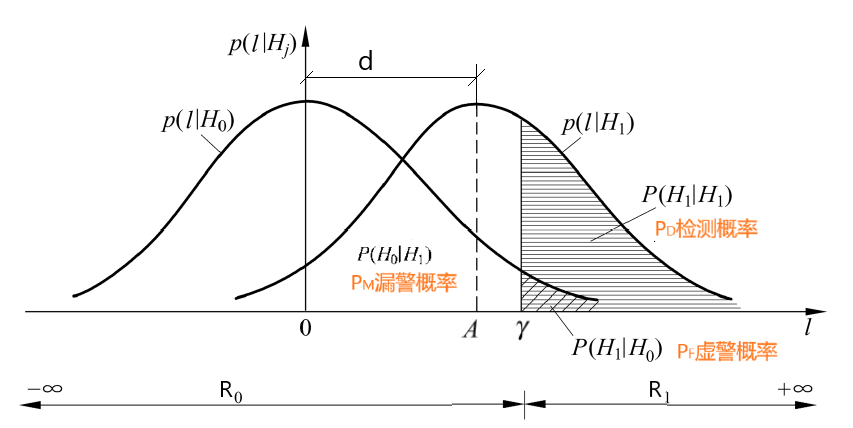
\includegraphics[scale=0.18]{R0R1}\\
	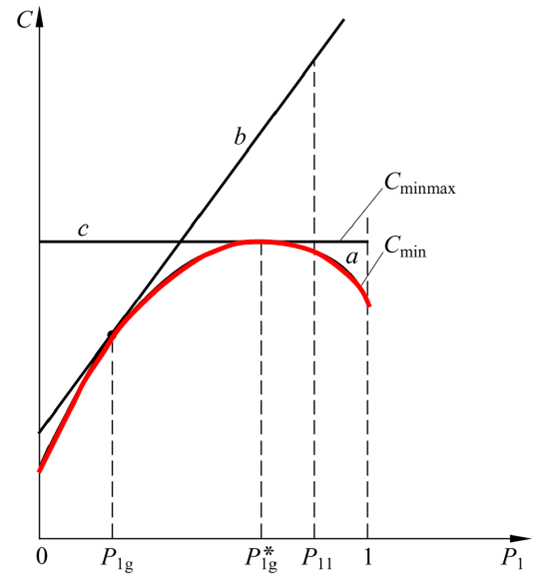
\includegraphics[scale=0.25]{C-P1}
\end{columns}
\end{frame}






